Discriminante lineal de Fisher es un método utilizado en estadística, reconocimiento de patrones y aprendizaje de máquinas para encontrar una combinación lineal de rasgos que caracterizan o separan dos o más clases de objetos o eventos. La combinación resultante puede ser utilizada como un clasificador lineal, o, más comúnmente, para la reducción de dimensiones antes de la posterior clasificación.

\subsection{Ejercicio 1}

Implementación del discriminante lineal de Fisher para 2 clases. En este caso lo que hacemos es buscar el mejor vector posible que maximize la separacion entre las dos clases ingresadas (a este vector lo llamaremos $W$). Luego proyectamos los datos en dicho vector, reduciendo su dimensión de dos a una, lo que facilita la posterior clasificacion.
\\
Uso de la funcion $Fisher(X)$ creada en matlab:\\
Input:
\begin{itemize}
	\item $X$: Matriz de $(NxDxC)$ con los datos a analizar, donde:\\
	\begin{itemize}
	\item	$N$: Cantidad de datos.\\
	\item	$D$: Dimensión de los datos (En este caso 2).\\     
	\item	$C$: Cantidad de clases (En este caso 2).\\
	\end{itemize}
\end{itemize}

\subsubsection{Resultados e Imágenes}

\begin{figure}[ht!]
\centering
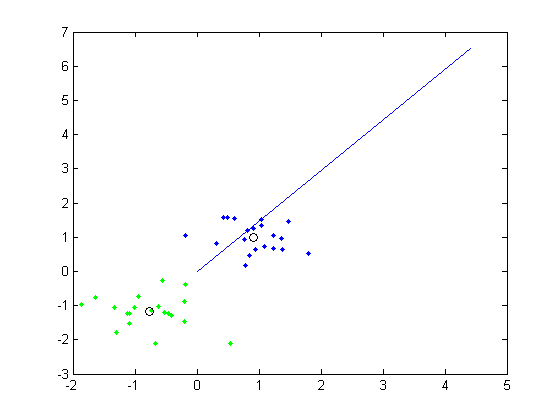
\includegraphics[width=120mm]{img/tp4/ej1-1.png}
\caption{Conjuntos de datos en dos dimensiónes y $W$.}
\end{figure}

\begin{figure}[ht!]
\centering
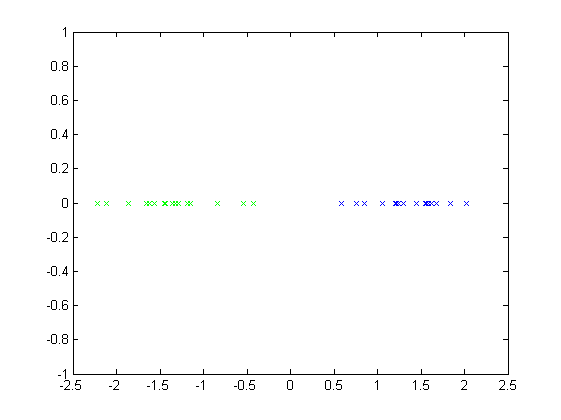
\includegraphics[width=120mm]{img/tp4/ej1-2.png}
\caption{Conjuntos de datos ya proyectados en $W$.}
\end{figure}

\subsection{Ejercicio 2}

Implementación del discriminante lineal de Fisher para 3 o más clases de datos. En este caso, a diferencia del anterior, como los datos de entrada tienen más de dos dimensiónes lo que hacemos es decrementar una a una la dimensión hasta llegar a uno. Otro cambio es el vector $W$ que utilizamos en el punto anterior para proyectar los datos, este ira variando segun la dimensión. Por ejemplo, si se trabaja con datos en tres dimensiónes este vector seria un plano.\\


Uso de la funcion $FDA(X,Y,r)$ creada en matlab:\\

$[Z,W]=FDA(X,Y,r)$\\

Input:
	\begin{itemize}
	\item$X$: Matriz de $(DxN)$ con los datos a analizar, donde:\\
		\begin{itemize}
		\item$D$: Dimensión de los datos.\\
		\item$N$: Cantidad de datos. \\
		\end{itemize}
	\item$Y$: Vector con etiqueta de la clase para cada dato.\\
	\item$r$: Dimensión a la cual queremos llevar nuestros datos.\\
	\end{itemize}
   
Output:
	\begin{itemize}
	\item$W$: $(Dxr)$ matriz de transformación.\\
	\item$Z$: $(rxN)$ matriz con los datos reducida su dimensión.\\
	\end{itemize}
 
\subsubsection{Resultados e Imágenes}

\begin{figure}[ht!]
\centering
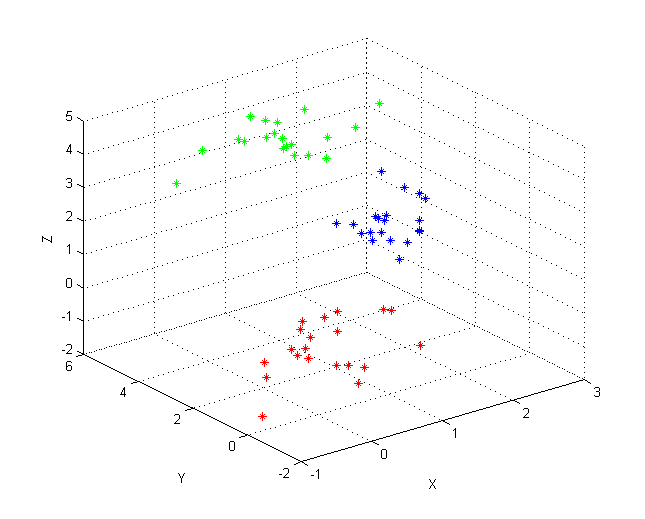
\includegraphics[width=120mm]{img/tp4/ej2-1.png}
\caption{Conjuntos de datos en tres dimensiónes.}
\end{figure}

\begin{figure}[ht!]
\centering
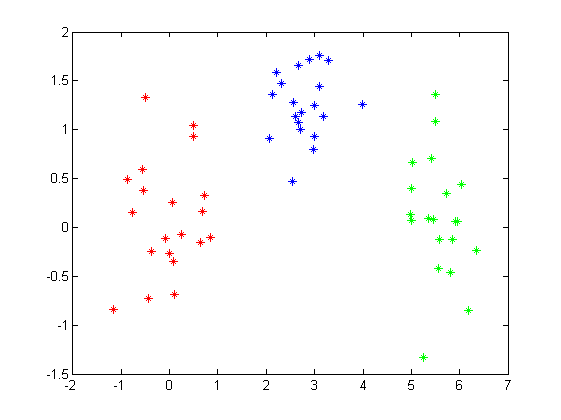
\includegraphics[width=120mm]{img/tp4/ej2-2.png}
\caption{Conjuntos de datos proyectados en $W$(plano).}
\end{figure}

\begin{figure}[ht!]
\centering
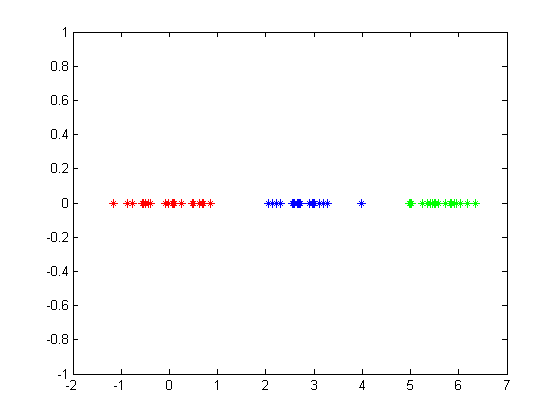
\includegraphics[width=120mm]{img/tp4/ej2-3.png}
\caption{Conjuntos de datos proyectados en $W$(vector).}
\end{figure}

\subsection{Ejercicio 3}

Aplicación de los programas desarrollados en los dos puntos anteriores a datos Gaussianos multidimensionales
isotrópicos.

\subsubsection{Resultados e Imágenes, 2 Clases}

Clase 1 (Azul): 45 elementos, $\mu$ = [1;1], $\sigma$ = [0.25 0 ; 0 0.25]\\
Clase 2 (Verde): 45 elementos, $\mu$ = [-1;-1], $\sigma$ = [0.25 0 ; 0 0.25]\\

\begin{figure}[ht!]
\centering
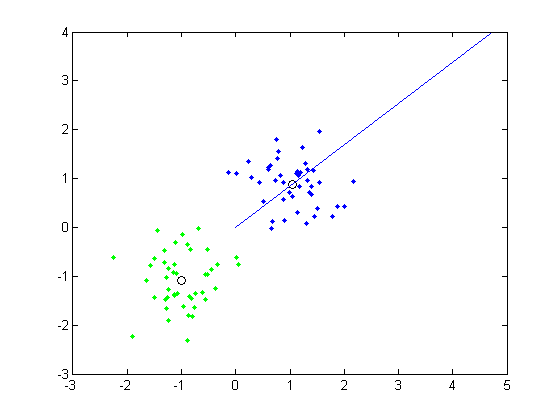
\includegraphics[width=120mm]{img/tp4/ej3-1.png}
\caption{Conjuntos de datos en dos dimensiónes y $W$.}
\end{figure}

\begin{figure}[ht!]
\centering
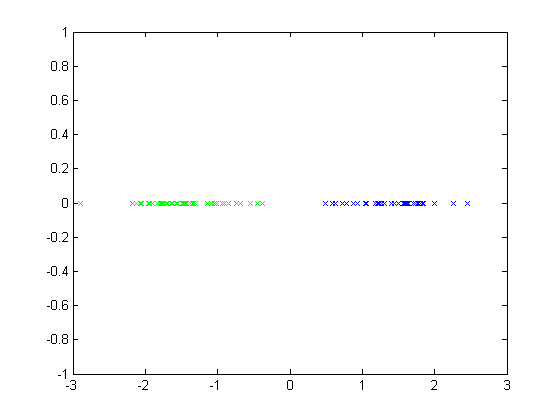
\includegraphics[width=120mm]{img/tp4/ej3-2.png}
\caption{Conjuntos de datos ya proyectados en $W$.}
\end{figure}

\subsubsection{Resultados e Imágenes, 3 Clases}

Clase 1 (Rojo): 45 elementos, $\mu$ = [0;0;0], $\sigma$ = [0.25 0 0 ; 0 0.25 0 ; 0 0 0.25]\\
Clase 2 (Azul): 45 elementos, $\mu$ = [2;2;2], $\sigma$ = [0.25 0 0 ; 0 0.25 0 ; 0 0 0.25]\\
Clase 3 (Verde): 45 elementos, $\mu$ = [1;4;4], $\sigma$ = [0.25 0 0 ; 0 0.25 0 ; 0 0 0.25]

\begin{figure}[ht!]
\centering
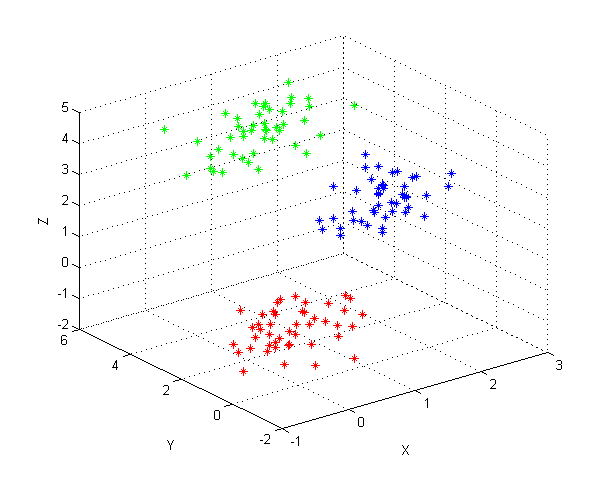
\includegraphics[width=120mm]{img/tp4/ej3-3.png}
\caption{Conjuntos de datos en tres dimensiónes.}
\end{figure}

\begin{figure}[ht!]
\centering
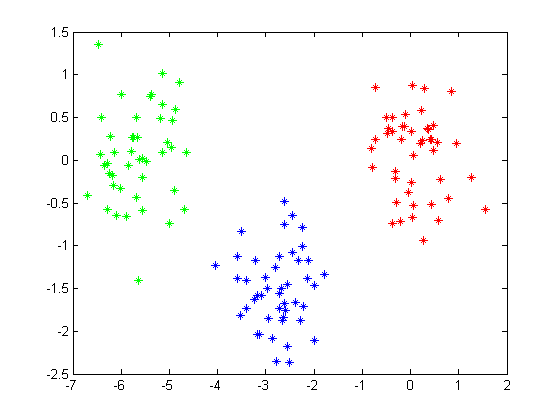
\includegraphics[width=120mm]{img/tp4/ej3-4.png}
\caption{Conjuntos de datos ya proyectados en $W$(plano).}
\end{figure}

\begin{figure}[ht!]
\centering
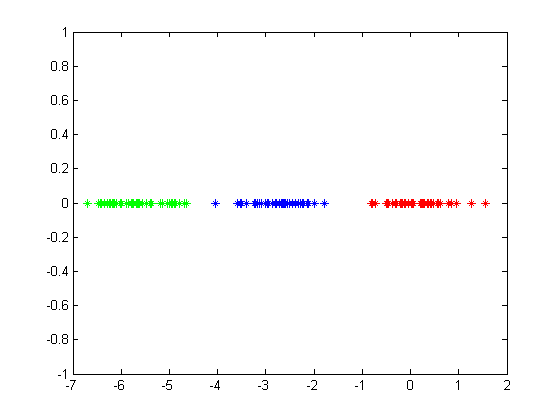
\includegraphics[width=120mm]{img/tp4/ej3-5.png}
\caption{Conjuntos de datos ya proyectados en $W$(vector).}
\end{figure}

\subsection{Ejercicio 4}

Luego de probar varios grados de separacion llegamos a la conclusion de que existen tres casos significativos.\\
Utilizamos dos clases con a datos Gaussianos multidimensionales
isotrópicos. Una clase fija, de 45 elementos, $\mu$ = [0;0] y $\sigma$ = [0.25 0 ; 0 0.25] y una segunda clase que varia en cada caso.

\subsubsection{Resultados e Imágenes}

El primer caso es el optimo, en el cual ambas clases tienen medias muy distantes y los datos en ningun momento se mezclan. Esto permite que el discriminante lineal de Fisher retorne un resultado muy facil de clasificar.\\
Segunda clase: $\mu$ = [2;2] y $\sigma$ = [0.25 0 ; 0 0.25]

\begin{figure}[ht!]
\centering
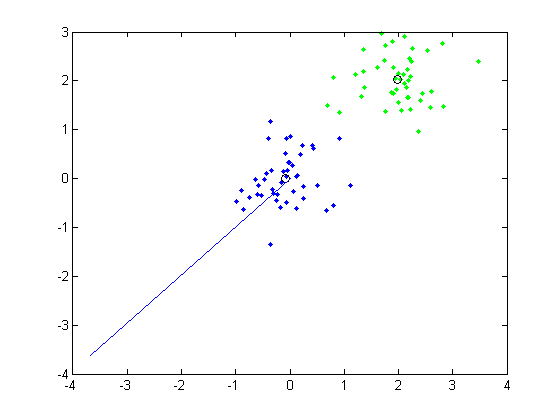
\includegraphics[width=120mm]{img/tp4/ej4-1.png}
\caption{Conjuntos de datos en dos dimensiónes y $W$.}
\end{figure}

\begin{figure}[ht!]
\centering
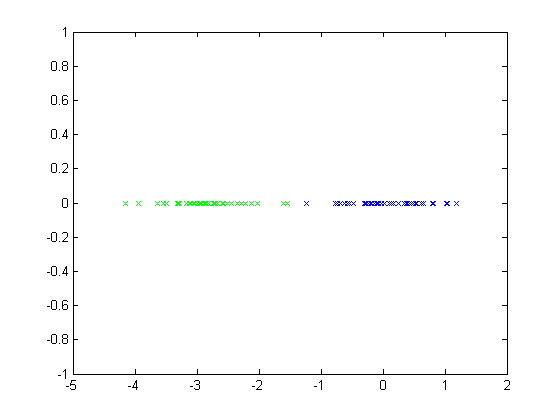
\includegraphics[width=120mm]{img/tp4/ej4-2.png}
\caption{Conjuntos de datos ya proyectados en $W$.}
\end{figure}

El segundo es aquel en el cual las medias son cercanas y algunos de sus elementos se mezclan. Esto hace que el discriminante lineal de Fisher retorne un resultado que al clasificarlo no es perfecto, pero se aproxima bastante.\\
Segunda clase: $\mu$ = [0.7;0.7] y $\sigma$ = [0.25 0 ; 0 0.25]

\begin{figure}[ht!]
\centering
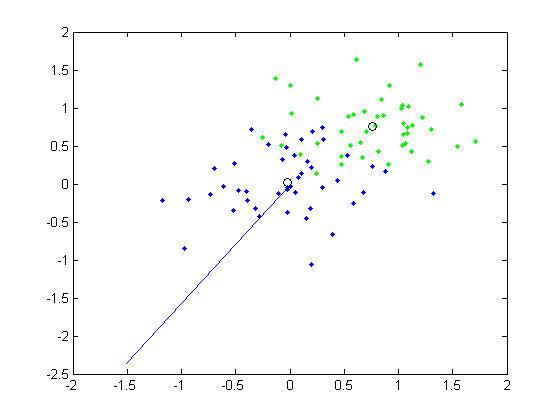
\includegraphics[width=120mm]{img/tp4/ej4-3.png}
\caption{Conjuntos de datos en dos dimensiónes y $W$.}
\end{figure}

\begin{figure}[ht!]
\centering
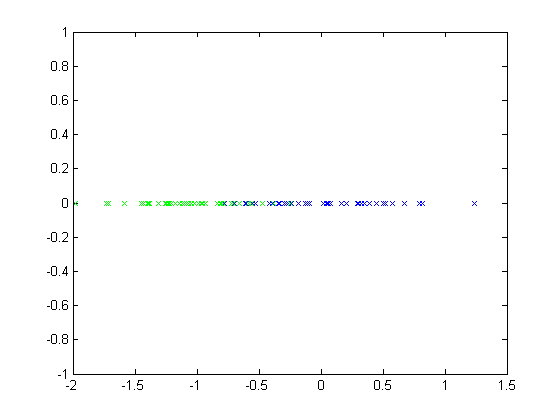
\includegraphics[width=120mm]{img/tp4/ej4-4.png}
\caption{Conjuntos de datos ya proyectados en $W$.}
\end{figure}

El tercero es aquel en el cual las medias son muy similares o iguales y la mayoria de elementos se mezclan. Esto hace que el discriminante lineal de Fisher retorne un resultado imposible de clasificar. Este metodo no es eficaz para esta clase de datos.\\
Segunda clase: $\mu$ = [0;0] y $\sigma$ = [0.25 0 ; 0 0.25]

\begin{figure}[ht!]
\centering
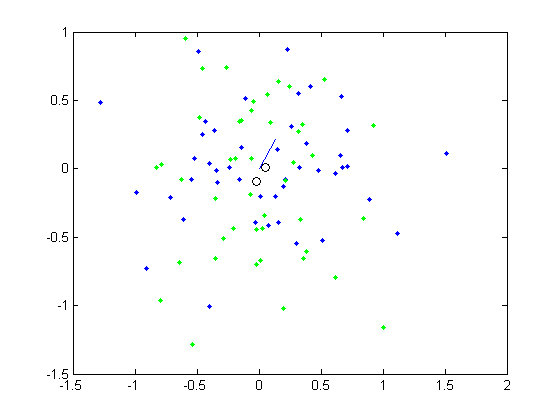
\includegraphics[width=120mm]{img/tp4/ej4-5.png}
\caption{Conjuntos de datos en dos dimensiónes y $W$.}
\end{figure}

\begin{figure}[ht!]
\centering
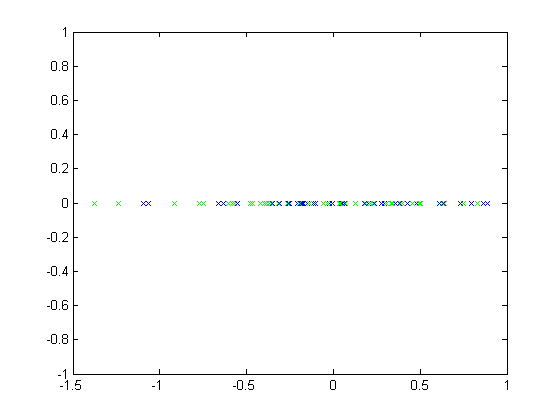
\includegraphics[width=120mm]{img/tp4/ej4-6.png}
\caption{Conjuntos de datos ya proyectados en $W$.}
\end{figure}
